
\chapter{MATHEMATICAL BACKGROUND}

This chapter introduces the mathematical foundations of the methods studied in this work. Section~\ref{sec:boussinesq} presents the Boussinesq system and the limiting wave-equation regime. Section~\ref{sec:pseudospectral} develops the pseudospectral numerical method used to generate reference solutions. Sections~\ref{sec:neural_networks} and~\ref{sec:neural_operators} introduce, respectively, the neural network and neural operator architectures studied in this work.

% ---------------------------------------------------------------
\section{The Boussinesq System}
\label{sec:boussinesq}

The Boussinesq system is a weakly nonlinear, weakly dispersive model governing the coupled evolution of two scalar fields in shallow water: the free surface elevation $\eta(x,t)$ and the depth-averaged horizontal velocity $u(x,t)$, both depending on position $x$ and time $t$. In the one-dimensional, spatially periodic setting studied in this work, the system reads
\begin{subequations}\label{eq:boussinesq}
    \begin{align}
        \eta_t + u_x + \alpha\,(\eta u)_x &= 0, \label{eq:bous1} \\[4pt]
        u_t - \frac{\beta}{3}\,u_{xxt} + \eta_x + \alpha\,u u_x &= 0, \label{eq:bous2}
    \end{align}
\end{subequations}
on the spatial domain $x \in [-L, L]$, where $\alpha \geq 0$ is the nonlinearity parameter, $\beta > 0$ is the dispersion parameter, and $L > 0$ is the domain half-length. The two coefficients weigh the competing effects the model balances: $\alpha$ scales the nonlinear terms $(\eta u)_x$ and $u u_x$, which steepen the wave, while $\beta$ scales the dispersive term $u_{xxt}$, which spreads it. This nondimensional form follows equation~(3.1) of \textcite{martins2023} (see also \textcite{martins2024}).

The system~\eqref{eq:boussinesq} is solved throughout this work from a single solitary profile at rest,
\begin{equation}\label{eq:initial_condition}
    \eta(x,0) = A\,\operatorname{sech}^2(x), \qquad u(x,0) = 0,
\end{equation}
where $A > 0$ is the initial amplitude and $\operatorname{sech}(z) = 2/(e^z + e^{-z})$ is the hyperbolic secant. This places one crest at the centre $x = 0$ of an otherwise flat surface, with zero initial velocity, as drawn in Figure~\ref{fig:soliton_profile}.

\begin{figure}[h!]
    \centering
    
\includegraphics[width=\textwidth]{setup/soliton_profile.png}
    \caption{Initial condition $\eta(x,0) = A\operatorname{sech}^2(x)$ for $A = 1$.}
    \label{fig:soliton_profile}
    \autoriapropria
\end{figure}

\subsection{Recovering the Wave Equation}
\label{subsec:wave_eq}

When both coefficients vanish, $\alpha = \beta = 0$, the nonlinear and the dispersive terms disappear together and the Boussinesq system reduces to:
\begin{align}
    \eta_t + u_x &= 0, \label{eq:wave1} \\
    u_t + \eta_x &= 0. \label{eq:wave2}
\end{align}
The two fields decouple into a single scalar equation. Differentiating~\eqref{eq:wave1} with respect to $t$ gives
\begin{equation}\label{eq:wave_dt}
    \eta_{tt} + u_{xt} = 0,
\end{equation}
and differentiating~\eqref{eq:wave2} with respect to $x$ gives
\begin{equation}\label{eq:wave_dx}
    u_{tx} + \eta_{xx} = 0.
\end{equation}
Since $u_{xt} = u_{tx}$, subtracting~\eqref{eq:wave_dx} from~\eqref{eq:wave_dt} cancels the mixed derivative and leaves
\begin{equation*}
    \eta_{tt} - \eta_{xx} = 0,
\end{equation*}
that is, the wave equation for $\eta$,
\begin{equation}\label{eq:wave_eq}
    \eta_{tt} = \eta_{xx}.
\end{equation}
In an analogous manner, differentiating~\eqref{eq:wave2} with respect to $t$ and~\eqref{eq:wave1} with respect to $x$, the same cancellation leaves $u_{tt} - u_{xx} = 0$, so $u$ obeys the same equation.

D'Alembert's formula \parencite{debnath2012} provides the general solution to~\eqref{eq:wave_eq}. Given initial data $\eta(x,0) = f(x)$ and $\eta_t(x,0) = g(x)$, the solution is
\begin{equation}\label{eq:dalembert}
    \eta(x,t) = \frac{f(x+t) + f(x-t)}{2}
            + \frac{1}{2}\int_{x-t}^{x+t} g(s)\,ds.
\end{equation}

We now apply this to the initial condition~\eqref{eq:initial_condition}. From~\eqref{eq:wave1}, $\eta_t(x,0) = -u_x(x,0) = 0$, so $f(x) = A\operatorname{sech}^2(x)$ and $g \equiv 0$. The integral in~\eqref{eq:dalembert} vanishes and the surface elevation evolves as
\begin{equation}\label{eq:dalembert_eta}
    \eta(x, t) = \frac{A}{2}\bigl[\operatorname{sech}^2(x+t) + \operatorname{sech}^2(x-t)\bigr].
\end{equation}
The initial bump of amplitude $A$ therefore splits into two counter-propagating pulses of amplitude $A/2$, travelling at speed $\pm 1$ without changing shape.

For $u$, from~\eqref{eq:wave2} we have $u_t(x,0) = -\eta_x(x,0)$, so $f \equiv 0$ and $g(x) = -\eta_x(x,0)$. The $f$ term vanishes in~\eqref{eq:dalembert}, leaving
\begin{equation*}
    u(x,t) = -\frac{1}{2}\int_{x-t}^{x+t} \eta_x(s,0)\,ds
            = -\frac{1}{2}\bigl[\eta(x+t,0) - \eta(x-t,0)\bigr],
\end{equation*}
and substituting $\eta(x,0) = A\operatorname{sech}^2(x)$,
\begin{equation}\label{eq:dalembert_u}
    u(x,t) = \frac{A}{2}\bigl[\operatorname{sech}^2(x-t) - \operatorname{sech}^2(x+t)\bigr].
\end{equation}
Any deviation from this wave-equation baseline in the full system~\eqref{eq:boussinesq} is attributable either to dispersion ($\beta > 0$) or to nonlinearity ($\alpha > 0$).

% ---------------------------------------------------------------
\section{Pseudospectral Method}
\label{sec:pseudospectral}

The pseudospectral method is applied here to the Boussinesq system~\eqref{eq:boussinesq} on the periodic spatial domain $\Omega = [-L, L]$. It transforms the two fields in space alone and leaves time as a separate evolution direction, which is the treatment an evolution equation asks for: taking the DFT along $x$ turns each spatial derivative into an algebraic multiplication, so the PDE collapses into a system of ordinary differential equations in time, one for every spatial frequency. The nonlinearity is what keeps the method from being purely spectral. A product of two fields is not the product of their spectra, so each nonlinear term is instead assembled by returning to the grid, multiplying pointwise there and transforming back. Alternating between the two representations in this way preserves the accuracy of the spatial derivatives while keeping the nonlinear coupling cheap to evaluate.

\subsection{Spatial Discretization and the Discrete Fourier Transform}
\label{subsec:dft}

The spatial domain $\Omega = [-L, L]$ of total length $2L$ is discretized into $N_x$ equispaced points:
\begin{equation*}
    x_j = -L + j\,\Delta x, \qquad \Delta x = \frac{2L}{N_x},
    \qquad j = 0, \ldots, N_x - 1.
\end{equation*}
The Discrete Fourier Transform (DFT) of a function $f$ sampled at these points is \parencite{trefethen2000}:
\begin{equation}\label{eq:dft}
    \hat{f}(k) = \sum_{j=0}^{N_x-1} f(x_j)\, e^{-2\pi i k j / N_x},
    \qquad k = -\tfrac{N_x}{2}, \ldots, \tfrac{N_x}{2} - 1,
\end{equation}
with its inverse, the Inverse Discrete Fourier Transform (IDFT), recovering the physical values:
\begin{equation}\label{eq:idft}
    f(x_j) = \frac{1}{N_x} \sum_{k} \hat{f}(k)\, e^{2\pi i k j / N_x}.
\end{equation}
The fundamental identity of the DFT with respect to differentiation is that, for a periodic function, the spatial derivative transforms into a pointwise multiplication \parencite{trefethen2000, engsigkarup2012}:
\begin{equation}\label{eq:dft_deriv_raw}
    \widehat{(f_x)}(k) = i \frac{\pi k}{L}\, \hat{f}(k), \quad
    \widehat{(f_{xx})}(k) = -\frac{\pi^2 k^2}{L^2}\, \hat{f}(k).
\end{equation}
This is in contrast to finite-difference methods, where the derivative carries a truncation error that shrinks with the grid spacing. Here the error enters at a different point. The identity~\eqref{eq:dft_deriv_raw} is an exact statement about the trigonometric interpolant of the sampled values, so what remains is the discrepancy between that interpolant and the function itself. For a smooth periodic function this discrepancy decays faster than any fixed power of $\Delta x$, which is the spectral accuracy the method is named for \parencite{trefethen2000}.

We define the wavenumber of mode $k$ on $[-L,L]$ as:
\begin{equation}\label{eq:xi_def}
    \xi_k \;:=\; \frac{\pi k}{L}.
\end{equation}
With this definition, the derivative identities read:
\begin{equation}\label{eq:dft_deriv}
    \widehat{(f_x)}(k) = i\,\xi_k\,\hat{f}(k), \qquad
    \widehat{(f_{xx})}(k) = -\xi_k^2\,\hat{f}(k).
\end{equation}

\subsection{Spectral Formulation of the Boussinesq System}
\label{subsec:spectral_bou}

To bring the Boussinesq system~\eqref{eq:boussinesq} into the Fourier domain, following the spectral formulation of \textcite{martins2023}, we apply the DFT to each equation and use the derivative identities~\eqref{eq:dft_deriv}. Equation~\eqref{eq:bous1}, treating $\widehat{(\eta u)}(k,t)$ as a given nonlinear term, becomes:
\begin{equation}\label{eq:eta_t_spectral}
    \hat{\eta}_t(k,t) = -i\,\xi_k\,\hat{u}(k,t)
    - \alpha\, i\,\xi_k\,\widehat{(\eta u)}(k,t).
\end{equation}
Equation~\eqref{eq:bous2} requires more care because of the $u_{xxt}$ term. Since spatial derivatives commute with the DFT:
\begin{equation*}
    \widehat{(u_{xxt})}(k,t) = -\xi_k^2\,\hat{u}_t(k,t).
\end{equation*}
Substituting into the DFT of~\eqref{eq:bous2}, with its nonlinear term written in the equivalent form $u u_x = \frac{1}{2}(u^2)_x$:
\begin{equation*}
    \hat{u}_t(k,t) + \frac{\beta}{3}\,\xi_k^2\,\hat{u}_t(k,t)
    + i\,\xi_k\,\hat{\eta}(k,t)
    + \alpha\, i\,\xi_k\,\widehat{\!\left(\tfrac{1}{2}u^2\right)}(k,t) = 0.
\end{equation*}
Collecting the $\hat{u}_t(k,t)$ terms on the left and solving algebraically:
\begin{equation}\label{eq:u_t_spectral}
    \hat{u}_t(k,t) = \frac{
        -i\,\xi_k\,\hat{\eta}(k,t)
        - \alpha\, i\,\xi_k\,\widehat{\!\left(\tfrac{1}{2}u^2\right)}(k,t)
    }{
        1 + \dfrac{\beta\,\xi_k^2}{3}
    }.
\end{equation}
The division in~\eqref{eq:u_t_spectral} is where the transform pays off. Isolating $u_t$ in~\eqref{eq:bous2} means inverting the operator $1 - \frac{\beta}{3}\frac{\partial^2}{\partial x^2}$, and on the grid that operator couples neighbouring nodes, so inverting it amounts to solving a linear system for all $N_x$ nodal values at every evaluation of the right-hand side. Under the DFT the same operator is diagonal, acting on mode $k$ as multiplication by $1 + \frac{\beta\,\xi_k^2}{3}$, and the inversion reduces to one division per mode.

Equations~\eqref{eq:eta_t_spectral} and~\eqref{eq:u_t_spectral} can be written jointly as a first-order ODE system in time for each fixed wavenumber $k \in \mathbb{Z}$:
\begin{equation}\label{eq:fourier_ode_k}
\begin{cases}
    \hat{\eta}_t(k,t) = -i\,\xi_k\,\hat{u}(k,t) - \alpha\,i\,\xi_k\,\widehat{(\eta u)}(k,t), \\[8pt]
    \hat{u}_t(k,t) = \dfrac{-i\,\xi_k\,\hat{\eta}(k,t) - \alpha\,i\,\xi_k\,\widehat{\!\left(\tfrac{1}{2}u^2\right)}\!(k,t)}{1 + \dfrac{\beta\,\xi_k^2}{3}}.
\end{cases}
\end{equation}
The PDE system~\eqref{eq:boussinesq}, two equations in $(x,t)$, is thus equivalent to an infinite family of two-dimensional ODE systems~\eqref{eq:fourier_ode_k}, one for each $k \in \mathbb{Z}$, coupled through the nonlinear terms.

The nonlinear terms $\widehat{(\eta u)}(k,t)$ and $\widehat{(\frac{1}{2}u^2)}(k,t)$ cannot be computed directly in Fourier space without a convolution sum, which costs $O(N_x^2)$. The pseudospectral approach avoids this by computing products in physical space. For $\widehat{(\eta u)}(k,t)$, the procedure is:
\begin{enumerate}
    \item recover $\eta(x_j)$ and $u(x_j)$ by applying the inverse DFT~\eqref{eq:idft};
    \item compute the product $(\eta u)_j = \eta(x_j)\cdot u(x_j)$ pointwise on the grid;
    \item apply the DFT~\eqref{eq:dft} to obtain $\widehat{(\eta u)}(k,t)$.
\end{enumerate}
Similarly, $\widehat{(\frac{1}{2}u^2)}(k,t)$ is obtained by the same three-step procedure with $u^2(x_j) = u(x_j)^2$, where $u(x_j) = \operatorname{IDFT}(\hat{u})(x_j)$; and $(\eta u)(x_j) = \operatorname{IDFT}(\hat{\eta})(x_j)\cdot\operatorname{IDFT}(\hat{u})(x_j)$. Since each DFT/IDFT costs $O(N_x \log N_x)$ via the Fast Fourier Transform (FFT), this pseudospectral strategy assembles each nonlinear term in $O(N_x \log N_x)$ instead of $O(N_x^2)$.

The nonlinear term of~\eqref{eq:bous2} fits this procedure only in the form it was given in~\eqref{eq:u_t_spectral}. Since $u u_x = \frac{1}{2}(u^2)_x$, the two forms are equivalent, but only the second is a product of a field with itself: recovering $u$ on the grid, squaring it pointwise and transforming back costs one inverse and one forward transform, whereas $u u_x$ would require recovering $u$ and $u_x$ separately before multiplying them. Both forms appear in this work. The solver uses $\frac{1}{2}(u^2)_x$ for exactly this reason, while the physics-informed network of Section~\ref{subsec:pinn} differentiates $u u_x$ directly by automatic differentiation, where the products are never assembled on a grid and the distinction carries no cost.

\subsection{Time Evolution via Runge-Kutta 4}
\label{subsec:rk4}

Collecting the two spectral fields into a single state vector $\hat{Y}(t) = \bigl(\hat{\eta}(k,t),\, \hat{u}(k,t)\bigr)$, the system~\eqref{eq:fourier_ode_k} takes the standard form of an initial value problem for a system of ordinary differential equations,
\begin{equation}\label{eq:ode_form}
    \hat{Y}_t(t) = F\bigl(\hat{Y}(t)\bigr),
\end{equation}
where the pseudospectral right-hand side operator $F$ is the map
\begin{equation*}
    F\!\left(\hat{\eta},\hat{u}\right)(k)
    \;=\;
    \begin{pmatrix}
        -i\,\xi_k\,\hat{u}(k)
        - \alpha\,i\,\xi_k\,\widehat{(\eta u)}(k) \\[6pt]
        \dfrac{
            -i\,\xi_k\,\hat{\eta}(k)
            - \alpha\,i\,\xi_k\,\widehat{\!\left(\tfrac{1}{2}u^2\right)}\!(k)
        }{
            1 + \dfrac{\beta\,\xi_k^2}{3}
        }
    \end{pmatrix},
\end{equation*}
whose two components are $\hat{\eta}_t$ and $\hat{u}_t$ as given by equations~\eqref{eq:eta_t_spectral}--\eqref{eq:u_t_spectral}, with the nonlinear terms assembled by the pseudospectral procedure above. In the form~\eqref{eq:ode_form} the problem is what any explicit one-step integrator expects, and time evolution uses the classical fourth-order Runge-Kutta (RK4) scheme \parencite{suli2003, burden2011}. Given the state $\hat{Y}_n = (\hat{\eta}^n, \hat{u}^n)$ at time $t_n$, the four stage evaluations $\kappa_1, \kappa_2, \kappa_3, \kappa_4$ and the update to $t_{n+1} = t_n + \Delta t$ are:
\begin{align*}
    \kappa_1 &= F(\hat{Y}_n), \\
    \kappa_2 &= F\!\left(\hat{Y}_n + \tfrac{\Delta t}{2}\, \kappa_1\right), \\
    \kappa_3 &= F\!\left(\hat{Y}_n + \tfrac{\Delta t}{2}\, \kappa_2\right), \\
    \kappa_4 &= F\!\left(\hat{Y}_n + \Delta t\, \kappa_3\right), \\
    \hat{Y}_{n+1}  &= \hat{Y}_n + \frac{\Delta t}{6}\,(\kappa_1 + 2\,\kappa_2 + 2\,\kappa_3 + \kappa_4).
\end{align*}
At each stage, the intermediate state is decoded to physical space to assemble the nonlinear products, then encoded back to Fourier space to evaluate the spectral derivatives. This split between physical-space products and Fourier-space derivatives is what characterizes the pseudospectral method.

% ---------------------------------------------------------------
\subsection{Training Dataset}
\label{sec:dataset}

The numerical experiments in this work vary only the PDE parameters $(\alpha,\beta)$ while keeping the initial condition fixed at~\eqref{eq:initial_condition}. The models are therefore trained and evaluated on the dataset
\begin{equation}\label{eq:dataset}
    \mathcal{S} = \bigl\{\bigl((\alpha_i,\beta_i),\,(\eta_i,u_i)\bigr)\bigr\}_{i=1}^{M},
\end{equation}
where $(\alpha_i,\beta_i)$ are the nonlinearity and dispersion parameters for the $i$-th sample, and $(\eta_i,u_i)$ is the corresponding space-time solution obtained from the pseudospectral solver of Section~\ref{sec:pseudospectral} with those parameters and the shared initial condition~\eqref{eq:initial_condition}.

% ---------------------------------------------------------------
\section{Neural Networks}
\label{sec:neural_networks}

This section introduces the neural network architectures central to this work, together with the theory that explains how they train. We begin with the Multilayer Perceptron, the base model underlying every architecture studied here. We then develop the Neural Tangent Kernel. That kernel is the tool we use to analyse the spectral bias a network produces when it is fitted to data sampled on a regular grid. Finally we turn to Physics-Informed Neural Networks. There we show that the same kernel analysis carries over to the physics-informed setting, where spectral bias is a well-documented obstacle.

\subsection{Multilayer Perceptrons}
\label{subsec:mlp}

In this work, we focus on Multilayer Perceptrons (MLPs), popularized by \textcite{rumelhart1986}. These networks are compositions of affine transformations parametrized by tunable weights and biases, separated by nonlinear activations, where an optimization process fits the network to a dataset.

Given a labeled dataset ${\{(x_i, u_i)\}}_{i=1}^{N}$, the objective is to fit the function $u_{\theta}(x)$ by minimizing a loss function, here the Mean Squared Error (MSE). With $\|\cdot\|$ denoting the Euclidean norm, the unconstrained optimization problem is:
\begin{equation}
    \mathcal{L}_{\text{MLP}}(\theta) = \frac{1}{N} \sum_{i=1}^{N} \| u_{\theta}(x_i) - u_i \|^2. \label{eq:data_loss_nn}
\end{equation}
The MLP $u_\theta: \mathbb{R}^{d_{\mathrm{in}}} \to \mathbb{R}^{d_{\mathrm{out}}}$ is defined by the composition:
\begin{align}
    h^{(0)}       &= x \in \mathbb{R}^{d_{\mathrm{in}}}, \label{eq:input}                                                                 \\
    h^{(l)}       &= \sigma \left( W^{(l)} h^{(l-1)} + b^{(l)} \right) \in \mathbb{R}^{N_{\mathrm{MLP}}},
                   \quad l = 1, \dots, L_{\mathrm{MLP}}-1, \label{eq:hidden} \\
    u_{\theta}(x) &= W^{(L_{\mathrm{MLP}})} h^{(L_{\mathrm{MLP}}-1)} + b^{(L_{\mathrm{MLP}})} \in \mathbb{R}^{d_{\mathrm{out}}}. \label{eq:output}
\end{align}
\noindent where:
\begin{itemize}
    \item $L_{\mathrm{MLP}} \in \mathbb{N}$ is the number of layers and $N_{\mathrm{MLP}} \in \mathbb{N}$ the number of neurons per hidden layer;
    \item $W^{(l)} \in \mathbb{R}^{N_{\mathrm{MLP}} \times N_{\mathrm{MLP}}}$ and $b^{(l)} \in \mathbb{R}^{N_{\mathrm{MLP}}}$ are the weight matrix and bias vector at layer $l$, with $W^{(1)} \in \mathbb{R}^{d_{\mathrm{in}} \times N_{\mathrm{MLP}}}$ and $W^{(L_{\mathrm{MLP}})} \in \mathbb{R}^{N_{\mathrm{MLP}} \times d_{\mathrm{out}}}$ adapted at the boundaries;
    \item $\sigma : \mathbb{R} \to \mathbb{R}$ is a sigmoidal activation function applied elementwise, satisfying $\sigma(t) \to 1$ as $t \to +\infty$ and $\sigma(t) \to 0$ as $t \to -\infty$;
    \item $\theta = \{W^{(l)}, b^{(l)}\}_{l=1}^{L_{\mathrm{MLP}}}$ denotes all trainable parameters.
\end{itemize}

If the activation function is sigmoidal, MLPs are universal approximators: they can approximate any continuous function on a compact domain to arbitrary precision \parencite{cybenko1989}.

In Figure~\ref{fig:MLP_depiction}, we show a common depiction of the neural network. Here the input vector is the pair $(x,t) \in \mathbb{R}^2$ and the output is $(\eta_{\theta}(x,t), u_{\theta}(x,t)) \in \mathbb{R}^2$.

\begin{figure}[h!]
    \centering
    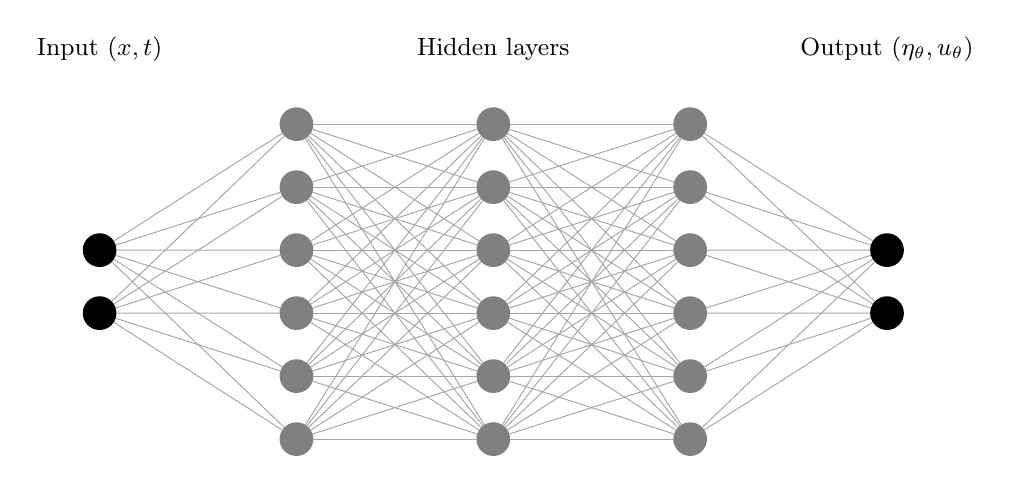
\begin{tikzpicture}[
            x=1cm,
            y=1cm,
            nnnode/.style={circle, draw, line width=0.8pt, minimum size=0.40cm, inner sep=0pt},
            inout/.style={nnnode, fill=black, draw=black},
            hidden/.style={nnnode, fill=gray, draw=gray},
            conn/.style={draw=gray!70, line width=0.35pt}
        ]
        \node[inout] (x1) at (0,-2.4) {};
        \node[inout] (x2) at (0,-3.2) {};
        \node at (0,0.15) {\small Input $(x,t)$};
        \foreach \i in {1,...,6} { \node[hidden] (h1_\i) at (2.5,-0.8*\i) {}; }
        \foreach \i in {1,...,6} { \node[hidden] (h2_\i) at (5.0,-0.8*\i) {}; }
        \node at (5.0,0.15) {\small Hidden layers};
        \foreach \i in {1,...,6} { \node[hidden] (h3_\i) at (7.5,-0.8*\i) {}; }
        \node[inout] (out1) at (10.0,-2.4) {};
        \node[inout] (out2) at (10.0,-3.2) {};
        \node at (10.0,0.15) {\small Output $(\eta_{\theta}, u_{\theta})$};
        \foreach \j in {1,...,6} {
            \draw[conn] (x1) -- (h1_\j);
            \draw[conn] (x2) -- (h1_\j);
        }
        \foreach \i in {1,...,6} {
            \foreach \j in {1,...,6} {
                \draw[conn] (h1_\i) -- (h2_\j);
                \draw[conn] (h2_\i) -- (h3_\j);
            }
        }
        \foreach \i in {1,...,6} {
            \draw[conn] (h3_\i) -- (out1);
            \draw[conn] (h3_\i) -- (out2);
        }
    \end{tikzpicture}
    \caption{Example of MLP architecture of input $(x, t)$, with $L_{\mathrm{MLP}}=3$ hidden layers and $N_{\mathrm{MLP}}=6$ neurons per layer.}
    \label{fig:MLP_depiction}
    \autoriapropria
\end{figure}

\subsection{Gradient Flow}
\label{subsec:grad_flow}

The analysis of the following sections is carried out on the continuous-time limit of gradient descent, the form in which the neural-tangent-kernel results this work relies on are stated \parencite{jacot2018, wang2022ntk}. This subsection derives that limit.

To understand how an MLP minimizes its data-fitting loss~\eqref{eq:data_loss_nn}, consider gradient descent with learning rate $\mu > 0$. Starting from an initialization $\theta^{(0)}$, each iteration updates the parameters by
\begin{equation}\label{eq:gd_discrete}
    \theta^{(k+1)} = \theta^{(k)} - \mu\,\nabla_\theta\mathcal{L}(\theta^{(k)}), \qquad k = 0, 1, 2, \ldots,
\end{equation}
where $\theta^{(k)}$ denotes the parameter vector after $k$ steps. Rearranging~\eqref{eq:gd_discrete} and dividing by the step size $\mu$ isolates the per-step increment as a difference quotient:
\begin{equation}\label{eq:gd_quotient}
    \frac{\theta^{(k+1)} - \theta^{(k)}}{\mu} = -\nabla_\theta\mathcal{L}(\theta^{(k)}).
\end{equation}
The left-hand side of~\eqref{eq:gd_quotient} already has the shape of a derivative: a difference of two parameter vectors divided by a spacing. It is not one yet. The index $k$ counts iterations and carries no unit of time, so there is nothing for the difference to be taken with respect to. Reading~\eqref{eq:gd_quotient} as the discretization of an ordinary differential equation therefore requires a new, continuous parameter along which the iterates can be laid out.

The idea is to regard the discrete sequence $\{\theta^{(k)}\}_{k=0}^{\infty}$ as samples of a smooth curve $\theta(\tau)$, read at a set of instants $\tau^{(k)}$,
\begin{equation}\label{eq:sampling}
    \theta^{(k)} = \theta(\tau^{(k)}),
\end{equation}
so that the recursion becomes a statement about $\theta(\tau)$ rather than about the index $k$. What remains is to fix the instants. The step size $\mu$ supplies their spacing: we assign to the $k$-th iterate the training-time stamp
\begin{equation}\label{eq:tau_k}
    \tau^{(k)} = k\mu, \qquad \text{so that} \qquad \tau^{(k+1)} - \tau^{(k)} = \mu,
\end{equation}
which places successive iterates $\mu$ apart along a time axis $\tau$ and gives $\theta^{(k+1)} = \theta(\tau^{(k)} + \mu)$. Substituting into the left-hand side of~\eqref{eq:gd_quotient} recasts it as a forward finite-difference quotient of $\theta$ in $\tau$:
\begin{equation}\label{eq:fd_quotient}
    \frac{\theta(\tau^{(k)} + \mu) - \theta(\tau^{(k)})}{\mu} = -\nabla_\theta\mathcal{L}\bigl(\theta(\tau^{(k)})\bigr).
\end{equation}
As the step size $\mu \to 0$, the spacing in~\eqref{eq:tau_k} shrinks to zero, the discrete stamps $\tau^{(k)}$ fill out a continuous variable $\tau$, and the left-hand side of~\eqref{eq:fd_quotient} converges to the derivative $d\theta/d\tau$ by definition of the derivative. The recursion thus becomes the gradient flow ODE:
\begin{equation}\label{eq:grad_flow}
    \frac{d\theta}{d\tau} = -\nabla_\theta \mathcal{L}(\theta), \qquad \theta(0) = \theta^{(0)}.
\end{equation}
The gradient flow~\eqref{eq:grad_flow} is a central object in optimization, and many standard first-order methods can be recovered as different time-discretization schemes of this same continuous trajectory. The discrete update~\eqref{eq:gd_discrete} is precisely the forward (explicit) Euler discretization of~\eqref{eq:grad_flow} with step size $\mu$ \parencite{suli2003, burden2011}, so gradient descent is just one numerical integrator for the flow; applying instead the backward (implicit) Euler scheme \parencite{suli2003} recovers the proximal gradient method \parencite{parikh2013}. Reading optimizers as discretizations of~\eqref{eq:grad_flow} thus organizes them into a single family, and it is the continuous flow that we analyze in what follows.

\subsection{Neural Tangent Kernel}
\label{subsec:ntk}

The kernel derived in this subsection was introduced by \textcite{jacot2018} and carried to the physics-informed setting by \textcite{wang2022ntk}; the derivation below follows their treatment, specialized to the data-fitting loss~\eqref{eq:data_loss_nn}. Consider the MLP fit to the dataset $\{(x_i,u_i)\}_{i=1}^{N}$ of Section~\ref{subsec:mlp}. Group the pointwise fitting errors into a single error vector:
\begin{equation}\label{eq:error_vector}
    e(\theta) =
    \begin{bmatrix}
        u_\theta(x_1) - u_1 \\
        \vdots \\
        u_\theta(x_{N}) - u_{N}
    \end{bmatrix}
    \in \mathbb{R}^{N}.
\end{equation}
Up to the constant factor $1/N$, the loss~\eqref{eq:data_loss_nn} is the squared norm of this vector, which we use in the form
\begin{equation}\label{eq:loss_quadratic}
    \mathcal{L}(\theta) = \frac{1}{2}\,\|e(\theta)\|^2 = \frac{1}{2}\sum_{i=1}^{N} e_i(\theta)^2,
\end{equation}
where $e_i(\theta) = u_\theta(x_i) - u_i$ is the $i$-th component of the error vector~\eqref{eq:error_vector}.
Define the Jacobian of the error vector with respect to the parameters:
\begin{equation}\label{eq:jacobian}
    J(\theta) = \frac{\partial e}{\partial\theta} \in \mathbb{R}^{N \times N_\theta},
    \qquad J_{ij} = \frac{\partial e_i}{\partial\theta_j},\quad i = 1,\ldots,N,\; j = 1,\ldots,N_\theta,
\end{equation}
where $N_\theta$ is the total number of trainable parameters. Each row $J_i = (J_{i1},\ldots,J_{iN_\theta}) \in \mathbb{R}^{N_\theta}$ is the parameter-gradient of the $i$-th residual. Since $\mathcal{L}$ is the quadratic form~\eqref{eq:loss_quadratic}, the $j$-th component of the loss gradient is:
\begin{equation}
    \frac{\partial \mathcal{L}}{\partial \theta_j}
    = \sum_{i=1}^{N} e_i(\theta)\,\frac{\partial e_i}{\partial \theta_j}
    = \sum_{i=1}^{N} J_{ij}\,e_i(\theta)
    = \bigl(J(\theta)^T e(\theta)\bigr)_j.
\end{equation}
Collecting all $j = 1,\ldots,N_\theta$ into a column vector:
\begin{equation}\label{eq:loss_grad}
    \nabla_\theta\mathcal{L} = J(\theta)^T\,e(\theta) \in \mathbb{R}^{N_\theta}.
\end{equation}
Substituting~\eqref{eq:loss_grad} into the gradient flow~\eqref{eq:grad_flow}:
\begin{equation}\label{eq:param_dynamics}
    \frac{d\theta}{d\tau} = -J(\theta)^T\,e(\tau).
\end{equation}
The error is written here as a function of $\tau$ rather than of $\theta$. The two notations denote the same object: along the flow the parameters are themselves a function of training time, so $e(\tau) := e(\theta(\tau))$, and it is this composition whose evolution we now track.
To find how the error vector itself evolves, differentiate each component $e_i(\theta(\tau))$ with respect to $\tau$ by the chain rule:
\begin{equation}
    \frac{de_i}{d\tau}
    = \sum_{j=1}^{N_\theta} \frac{\partial e_i}{\partial \theta_j}\,\frac{d\theta_j}{d\tau}
    = J_i(\theta)\cdot\frac{d\theta}{d\tau}.
\end{equation}
Stacking this identity for all $i = 1,\ldots,N$ into a matrix equation:
\begin{equation}
    \frac{de}{d\tau} = J(\theta)\,\frac{d\theta}{d\tau}.
\end{equation}
Substituting~\eqref{eq:param_dynamics}:
\begin{equation}\label{eq:ntk_dynamics}
    \frac{de}{d\tau}
    = J(\theta)\bigl(-J(\theta)^T e(\tau)\bigr)
    = -\underbrace{J(\theta)\,J(\theta)^T}_{K(\theta)\;\in\;\mathbb{R}^{N\times N}}\,e(\tau).
\end{equation}
The matrix $K(\theta) = J(\theta)J(\theta)^T$ is the empirical Neural Tangent Kernel (NTK) \parencite{jacot2018}. It is symmetric positive semi-definite by construction: for any $v \in \mathbb{R}^{N}$,
\begin{equation}
    v^T K(\theta)\, v = v^T J(\theta)\,J(\theta)^T v = \bigl\|J(\theta)^T v\bigr\|^2 \geq 0.
\end{equation}
The $(i,j)$ entry of $K(\theta)$ follows directly from expanding the matrix product $J(\theta)J(\theta)^T$:
\begin{equation}\label{eq:ntk_entry}
    K_{ij}(\theta)
    = \sum_{l=1}^{N_\theta} J_{il}(\theta)\,J_{jl}(\theta)
    = \sum_{l=1}^{N_\theta} \frac{\partial e_i}{\partial\theta_l}(\theta)\,\frac{\partial e_j}{\partial\theta_l}(\theta)
    = \nabla_\theta e_i(\theta)^T\,\nabla_\theta e_j(\theta).
\end{equation}
This is the inner product in $\mathbb{R}^{N_\theta}$ of the parameter gradients of the network output at the $i$-th and $j$-th training points, where $e_i = u_\theta(x_i) - u_i$. Hence $K(\theta) \in \mathbb{R}^{N \times N}$ is the Gram matrix of the network's sensitivities across the whole dataset, and equation~\eqref{eq:ntk_dynamics} shows that it alone governs how the fitting error evolves under gradient flow.

\subsection{Spectral Bias}
\label{subsec:spectral_bias}

The spectral bias (or frequency principle) is the empirical observation that neural networks trained by gradient-based methods reduce the low-frequency components of the error faster than the high-frequency ones \parencite{rahaman2019}. This section derives that phenomenon directly from the NTK dynamics established above. When the training points lie on a regular grid and the target function is periodic, the error admits a discrete Fourier representation, and one can ask how its frequency content is approximated along the training iterations. We first establish the decay in the eigenbasis of the NTK and then, by transforming to Fourier space, show that it is precisely the low frequencies that are resolved first.

For a network with a sufficiently large number of parameters, the Jacobian $J(\theta)$ changes negligibly during training, a regime known as lazy training \parencite{jacot2018, chizat2019, wang2022ntk}. The motivation for it is a scaling argument. In the wide-network limit the output at any point is an aggregate of many hidden units, each contributing a vanishing share of it as the width grows. An $O(1)$ change in the function is then reached by many parameters each moving very little, instead of a few moving a lot. Since the Jacobian is itself a function of the parameters, it barely moves either, and in the infinite-width limit it stays frozen at its value at initialization \parencite{jacot2018, chizat2019}. The networks trained here are finite, so this is an approximation, not an identity, and how far it holds is measured directly in Chapter~\ref{chap:results}. Writing $J_0 = J(\theta(0))$ and $K_0 = J_0 J_0^T$, the approximation $K(\theta(\tau)) \approx K_0$ turns equation~\eqref{eq:ntk_dynamics} into a linear ODE with constant coefficients:
\begin{equation}\label{eq:error_linear_ode}
    \frac{de}{d\tau} = -K_0\,e(\tau), \qquad e(0) = e_0.
\end{equation}
Written component-wise, the $i$-th row of this system is
\begin{equation}\label{eq:ntk_component}
    \frac{de_i}{d\tau} = -\sum_{j=1}^{N} K_0^{ij}\,e_j(\tau), \qquad i = 1,\ldots,N,
\end{equation}
where $K_0^{ij} = \nabla_{\theta_0} e_i^T\,\nabla_{\theta_0} e_j$ is the inner product, at initialization, of the parameter gradients of the network output at training points $x_i$ and $x_j$. The rate of change of the error at point $i$ is therefore a weighted sum of all current errors, with weights given by these pairwise kernel values. Through this coupling, the geometry of the sample grid and the architecture of the network jointly determine the convergence of every component.

Since $K_0 \in \mathbb{R}^{N \times N}$ is symmetric and positive semi-definite, the spectral theorem for symmetric matrices \parencite{strang2006, golub2013} guarantees a decomposition
\begin{equation}\label{eq:spectral_decomp}
    K_0 = V\,\Lambda\,V^T,
\end{equation}
where $V = [v_1 \mid \cdots \mid v_{N}]$ is an orthogonal matrix ($V^T V = I$) and
\begin{equation}
    \Lambda = \mathrm{diag}(\lambda_1,\ldots,\lambda_{N}), \qquad \lambda_1 \geq \lambda_2 \geq \cdots \geq \lambda_{N} \geq 0.
\end{equation}
Introduce the change of coordinates
\begin{equation}\label{eq:change_of_basis}
    c(\tau) = V^T e(\tau),
\end{equation}
so that, since $V$ is orthogonal, $e(\tau) = V c(\tau)$. Differentiating~\eqref{eq:change_of_basis} with respect to $\tau$ and substituting the ODE~\eqref{eq:error_linear_ode}:
\begin{equation}
    \frac{dc}{d\tau} = V^T \frac{de}{d\tau} = -V^T K_0\,e(\tau).
\end{equation}
Inserting $K_0 = V\Lambda V^T$ and $e(\tau) = Vc(\tau)$:
\begin{equation}
    \frac{dc}{d\tau}
    = -V^T\,(V\Lambda V^T)\,(Vc(\tau))
    = -(V^T V)\,\Lambda\,(V^T V)\,c(\tau)
    = -\Lambda\,c(\tau),
\end{equation}
using $V^T V = I$ at each step. Since $\Lambda$ is diagonal, this decouples into $N$ independent scalar equations:
\begin{equation}\label{eq:decoupled_ode}
    \frac{dc_k}{d\tau} = -\lambda_k\,c_k(\tau), \qquad k = 1,\ldots,N.
\end{equation}

Each equation in~\eqref{eq:decoupled_ode} is a first-order linear ODE with constant coefficient \parencite{boyce2012}. Separating the variables and integrating both sides from the initial state at $\tau = 0$ up to time $\tau$, with $s$ and $r$ as integration variables for the amplitude and the time,
\begin{equation}
    \int_{c_k(0)}^{c_k(\tau)} \frac{ds}{s}
    = -\lambda_k \int_0^{\tau} dr
    \qquad\Longrightarrow\qquad
    \ln\frac{|c_k(\tau)|}{|c_k(0)|} = -\lambda_k\,\tau.
\end{equation}
Exponentiating both sides yields the solution
\begin{equation}\label{eq:error_mode}
    c_k(\tau) = c_k(0)\,e^{-\lambda_k\tau},
\end{equation}
where $c_k(0) = v_k^T e_0$ is the projection of the initial error $e_0$ onto the $k$-th eigenvector of $K_0$. For $\lambda_k = 0$ the equation gives $c_k(\tau) = c_k(0)$ for all $\tau$: that eigendirection never decays.

Returning to the original coordinates via $e(\tau) = Vc(\tau)$:
\begin{equation}\label{eq:error_evolution}
    e(\tau) = \sum_{k=1}^{N} \bigl(v_k^T e_0\bigr)\,e^{-\lambda_k\tau}\,v_k.
\end{equation}
The error decomposes into $N$ independent eigendirections. Each eigenvector $v_k$ carries initial amplitude $v_k^T e_0$ and decays exponentially at rate $\lambda_k$: eigenvectors with large $\lambda_k$ are suppressed quickly, while those with small $\lambda_k$ persist throughout training. This per-eigendirection decay, each at the rate set by its eigenvalue, is the rigorous statement of spectral bias established by \textcite{cao2019}; the same spectral ordering governs generalization as the training set grows \parencite{bordelon2020}.

Equation~\eqref{eq:error_evolution} is the continuous flow; gradient descent takes finite steps, and its error evolution inherits the same eigenstructure in discrete form. The link between the two is the training-time stamp of~\eqref{eq:tau_k}: iterate $n$ sits at continuous time $\tau^{(n)} = n\mu$, so the iteration count and the training time are read off one another through
\begin{equation}\label{eq:tau_n_dictionary}
    \tau = n\mu, \qquad n = \tau/\mu.
\end{equation}

Section~\ref{subsec:grad_flow} read the update~\eqref{eq:gd_discrete} as forward Euler applied to the gradient flow in the parameters. The same statement is needed for the error, since that is what the analysis follows. There are two ways to obtain it: discretize the parameter update and then linearize, or linearize first, into the error equation~\eqref{eq:error_linear_ode}, and discretize that. Both give the same law.

Take the first. Gradient descent on the loss is
\[
    \theta^{(n+1)} = \theta^{(n)} - \mu\,\nabla_\theta\mathcal{L}\bigl(\theta^{(n)}\bigr).
\]
Under lazy training the Jacobian is frozen at $J_0$, so~\eqref{eq:loss_grad} gives $\nabla_\theta\mathcal{L}(\theta^{(n)}) = J_0^T e^{(n)}$ and the step is
\[
    \Delta\theta^{(n)} := \theta^{(n+1)} - \theta^{(n)} = -\mu\,J_0^T e^{(n)}.
\]
Expanding the error to first order in that displacement,
\[
    e^{(n+1)} = e^{(n)} + J_0\,\Delta\theta^{(n)} + O\bigl(\|\Delta\theta^{(n)}\|^2\bigr),
\]
and substituting the step,
\[
    e^{(n+1)} = e^{(n)} - \mu\,J_0 J_0^T e^{(n)}.
\]

Now the second. Equation~\eqref{eq:error_linear_ode} is already linear in $e$. The forward, or explicit, Euler scheme \parencite{suli2003, leveque2007} replaces its derivative at $\tau^{(n)}$ by a forward difference over one step of length $\mu$,
\[
    \left.\frac{de}{d\tau}\right|_{\tau^{(n)}} \approx \frac{e^{(n+1)} - e^{(n)}}{\mu},
\]
and evaluates the right-hand side at the current iterate,
\[
    \frac{e^{(n+1)} - e^{(n)}}{\mu} = -K_0\,e^{(n)}.
\]
Multiplying through by $\mu$,
\[
    e^{(n+1)} = e^{(n)} - \mu\,K_0\,e^{(n)}.
\]

Since $K_0 = J_0 J_0^T$, the two results are the same equation. Collecting terms gives the single-step law
\begin{equation}\label{eq:error_discrete_step}
    e^{(n+1)} = (I - \mu K_0)\,e^{(n)}.
\end{equation}
One gradient-descent step of size $\mu$ is one forward-Euler step of length $\mu$ on the error. Iterating from $e^{(0)} = e_0$ and diagonalizing with $K_0 = V\Lambda V^T$,
\begin{equation}\label{eq:error_discrete}
    e^{(n)} = (I - \mu K_0)^n e_0 = \sum_{k=1}^N \bigl(v_k^T e_0\bigr)\,(1 - \mu\lambda_k)^n\,v_k.
\end{equation}
The continuous solution reaches the same expression, one mode at a time. Evaluate the decay factor of~\eqref{eq:error_evolution} at $\tau = n\mu$ and split it across the $n$ steps,
\[
    e^{-\lambda_k\tau} = e^{-\lambda_k n\mu} = \bigl(e^{-\lambda_k\mu}\bigr)^n,
\]
then expand the per-step factor and truncate at first order in $\mu\lambda_k$ \parencite{burden2011},
\begin{equation}\label{eq:euler_truncation}
    e^{-\lambda_k\mu} = 1 - \mu\lambda_k + O\bigl((\mu\lambda_k)^2\bigr) \approx 1 - \mu\lambda_k.
\end{equation}
Substituting term by term carries~\eqref{eq:error_evolution} into~\eqref{eq:error_discrete}, so $(1-\mu\lambda_k)^n$ is the forward-Euler counterpart of $e^{-\lambda_k\tau}$. The two agree as the step vanishes with $\tau = n\mu$ held fixed,
\[
    \lim_{\mu \to 0}\, \bigl(1 - \mu\lambda_k\bigr)^{\tau/\mu} = e^{-\lambda_k\tau}.
\]

The same truncation constrains the step. Under the continuous flow every mode with $\lambda_k > 0$ decays for any $\mu > 0$. The discrete mode contracts only when its amplification factor is smaller than one in magnitude,
\begin{equation}\label{eq:euler_stability}
    \bigl| 1 - \mu\lambda_k \bigr| < 1
    \qquad\Longleftrightarrow\qquad
    0 < \mu\lambda_k < 2,
\end{equation}
which is the absolute-stability condition of the explicit Euler method \parencite{leveque2007, suli2003}. The product $\mu\lambda_k$ alone fixes how the $k$-th mode behaves, and it does so in four regimes. Below one, the factor lies in $(0,1)$ and the mode decays monotonically toward zero; at exactly one it vanishes and the mode is removed in a single step. Between one and two the factor is negative, so the mode still decays but flips sign at every step. Past two it exceeds one in magnitude and the mode grows without bound. A single step size therefore acts differently on every eigendirection of $K_0$.

Since $\lambda_1 = \lambda_{\max}$ is the largest eigenvalue, every mode stays stable only when the largest one does, which caps the learning rate at
\begin{equation}\label{eq:euler_bound}
    \mu < \frac{2}{\lambda_{\max}}.
\end{equation}
The minimal experiment of Section~\ref{sec:m_minimal} sets its step from this limit: rather than a nominal value, $\mu$ is fixed at a constant fraction of $2/\lambda_{\max}$ at every width, small enough to keep every mode in the monotone regime $\mu\lambda_k < 1$ while staying comparable across widths whose $\lambda_{\max}$ differ.

The same argument gives the time each mode needs. From~\eqref{eq:error_mode}, the amplitude of the $k$-th eigendirection at time $\tau$ is
\begin{equation}\label{eq:mode_amplitude}
    \bigl| c_k(\tau) \bigr| = \bigl| v_k^T e_0 \bigr|\, e^{-\lambda_k\tau}.
\end{equation}
Require it to fall below a target precision $\varepsilon > 0$,
\[
    \bigl| v_k^T e_0 \bigr|\, e^{-\lambda_k\tau} < \varepsilon,
\]
and divide by $\bigl| v_k^T e_0 \bigr| > 0$,
\[
    e^{-\lambda_k\tau} < \frac{\varepsilon}{\bigl| v_k^T e_0 \bigr|}.
\]
Taking logarithms preserves the inequality,
\[
    -\lambda_k\,\tau < \ln \frac{\varepsilon}{\bigl| v_k^T e_0 \bigr|},
\]
and dividing by $-\lambda_k < 0$ reverses it,
\[
    \tau > \frac{1}{\lambda_k}\,\ln \frac{\bigl| v_k^T e_0 \bigr|}{\varepsilon}.
\]
The minimum training time to resolve the $k$-th eigendirection to precision $\varepsilon$ is therefore
\begin{equation}\label{eq:training_time}
    \tau_k = \frac{1}{\lambda_k}\,\ln \frac{\bigl| v_k^T e_0 \bigr|}{\varepsilon}.
\end{equation}
The projection enters~\eqref{eq:training_time} through a logarithm and the eigenvalue through $1/\lambda_k$, so $\lambda_k$ sets the scale of $\tau_k$ while the projection only shifts it. Since $\lambda_1 \geq \lambda_2 \geq \cdots \geq \lambda_{N} \geq 0$, the times are ordered $\tau_1 \leq \tau_2 \leq \cdots \leq \tau_{N}$: higher-indexed eigendirections require more training time, in inverse proportion to their eigenvalue. \textcite{arora2019} reached similar conclusions from a discrete-time analysis of gradient descent, showing that the convergence speed of each eigenvector is governed by its eigenvalue and by the projection of the target onto that eigenvector.

The decomposition~\eqref{eq:error_evolution} is expressed in the eigenbasis $\{v_k\}_{k=1}^{N}$ of the NTK, which need not coincide with any physically meaningful basis. When the $N$ training points lie on a regular grid and the target is periodic, however, the natural basis is the Fourier one, and recasting the dynamics there shows that the decay is genuinely organized by frequency. Let $F \in \mathbb{C}^{N \times N}$ be the Fourier matrix, that is, the discrete Fourier transform (DFT) matrix with entries
\begin{equation}\label{eq:dft_matrix}
    F_{jl} = \frac{1}{\sqrt{N}}\,\omega^{jl}, \qquad \omega = e^{-2\pi \mathrm{i}/N}, \qquad j,l = 0,\ldots,N-1.
\end{equation}
With this normalization $F$ is unitary, $F^{*}F = I$, so that $F^{-1} = F^{*}$, where $F^{*}$ is the conjugate transpose \parencite{golub2013, strang2006}. Applying $F$ to the error vector yields its spectrum, with inverse transform $F^{-1}$:
\begin{equation}\label{eq:dft_error}
    \hat e(\tau) = F\,e(\tau), \qquad e(\tau) = F^{-1}\hat e(\tau) = F^{*}\hat e(\tau).
\end{equation}
In particular $\hat e_0 = F e_0$ is the spectrum of the initial error, the difference between the spectra of the initial network output and the target. Since $F$ is constant in $\tau$, applying it to the linearized dynamics~\eqref{eq:error_linear_ode} carries the error evolution into the frequency domain:
\begin{equation}\label{eq:fourier_dynamics}
    \frac{d\hat e}{d\tau}
    = F\,\frac{de}{d\tau}
    = -F K_0\,e(\tau)
    = -F K_0 F^{-1}\,\hat e(\tau).
\end{equation}
Inserting the eigendecomposition $K_0 = V\Lambda V^T$ from~\eqref{eq:spectral_decomp},
\begin{equation}\label{eq:fourier_diag}
    F K_0 F^{-1}
    = F V\,\Lambda\,V^T F^{-1}
    = (FV)\,\Lambda\,(FV)^{*}
    = (FV)\,\Lambda\,(FV)^{-1},
\end{equation}
where $V^T F^{-1} = V^{*} F^{*} = (FV)^{*}$ uses that $V$ is real orthogonal, and $(FV)^{*} = (FV)^{-1}$ uses that a product of unitary matrices is unitary. The columns of $FV$, namely the Fourier transforms $\{F v_k\}_{k=1}^{N}$ of the NTK eigenvectors, therefore diagonalize the frequency-domain dynamics. Defining the modal amplitudes $\tilde c(\tau) = (FV)^{-1}\hat e(\tau)$ and repeating the steps~\eqref{eq:change_of_basis}--\eqref{eq:error_mode} gives
\begin{equation}\label{eq:fourier_mode}
    \frac{d\tilde c_k}{d\tau} = -\lambda_k\,\tilde c_k(\tau)
    \qquad\Longrightarrow\qquad
    \tilde c_k(\tau) = \tilde c_k(0)\,e^{-\lambda_k\tau}.
\end{equation}
These are the same amplitudes as before: $\tilde c = (FV)^{-1}F e = V^{-1} e = V^T e = c$, the projection of the error onto the NTK eigenvectors, now read in Fourier space. Transforming back through~\eqref{eq:dft_error} yields the evolution of the error spectrum,
\begin{equation}\label{eq:fourier_evolution}
    \hat e(\tau) = \sum_{k=1}^{N} \bigl[(F v_k)^{*}\hat e_0\bigr]\, e^{-\lambda_k\tau}\,(F v_k).
\end{equation}
Equation~\eqref{eq:fourier_evolution} is the spectral-bias statement in the literal sense of the frequency spectrum: the error spectrum is a superposition of the transformed eigenvectors $F v_k$, each damped at its own rate $\lambda_k$. The frequencies resolved first are those carried by the eigenvectors with the largest eigenvalues; empirically these eigenvectors are smooth and concentrated in the low Fourier modes \parencite{rahaman2019, xu2019frequency}, so the low-frequency content of the error decays first while the high-frequency content persists.

To close, we specialize the initial condition. The weights of an MLP are drawn at random from a distribution centred at zero, so at small initialization scale $\theta_0 \approx 0$ and the network output $u_{\theta_0}$ is close to zero across the whole grid. Set against a target $u$ of order one, it is negligible. This is a common simplification in spectral-bias analyses, and under it the initial error is the target with opposite sign, as is its spectrum:
\begin{equation}\label{eq:init_spectrum}
    \hat e_0 = F\bigl(u_{\theta_0} - u\bigr) = \hat u_{\theta_0} - \hat u
    \approx -\,\hat u
    = -\begin{bmatrix} \hat u(0) \\ \vdots \\ \hat u(N-1) \end{bmatrix}.
\end{equation}
Substituting~\eqref{eq:init_spectrum} into~\eqref{eq:fourier_evolution} casts the dynamics as a reconstruction of the target frequency by frequency: each Fourier mode of $u$ is acquired at a rate set by the NTK eigenvalues, the smooth low-frequency content emerging first and the fine high-frequency detail last. This is the regime anticipated at the start of the section, a periodic target on a regular grid, in which the quality of the approximation can be tracked mode by mode along the training iterations. It is also the setting we implement: the minimal experiment of Chapter~\ref{chap:methodology} fits a single Boussinesq elevation profile on exactly such a grid, so that~\eqref{eq:init_spectrum} holds by construction and the mode-by-mode reconstruction can be measured against the prediction.

This last observation can be made quantitative. Taking the modulus of the modal amplitude~\eqref{eq:fourier_mode} isolates the magnitude of the $k$-th component along training,
\begin{equation}\label{eq:fourier_amplitude}
    |\tilde c_k(\tau)| = |\tilde c_k(0)|\,e^{-\lambda_k\tau},
    \qquad
    |\tilde c_k(0)| = |(F v_k)^{*}\hat e_0| \approx |(F v_k)^{*}\hat u|,
\end{equation}
where the last estimate uses the small-scale initialization~\eqref{eq:init_spectrum}, so that $|(F v_k)^{*}\hat u|$ measures how strongly the target overlaps with the $k$-th eigen-mode. Training, however, advances in discrete steps: by the construction of the gradient flow~\eqref{eq:tau_k}, the continuous time and the iteration count $n$ are related by $\tau = n\mu$, with $\mu$ the learning rate. Substituting $\tau = n\mu$ into~\eqref{eq:fourier_amplitude} and requiring the amplitude to fall below a target precision $\varepsilon > 0$,
\begin{equation}\label{eq:iteration_bound}
    |(F v_k)^{*}\hat u|\,e^{-\lambda_k n\mu} < \varepsilon
    \;\implies\;
    n > \frac{1}{\mu\,\lambda_k}\,\ln\frac{|(F v_k)^{*}\hat u|}{\varepsilon},
\end{equation}
gives an estimate of the number of gradient-descent iterations needed to resolve the $k$-th frequency:
\begin{equation}\label{eq:iteration_count}
    n_k = \left\lceil \frac{1}{\mu\,\lambda_k}\,\ln\frac{|(F v_k)^{*}\hat u|}{\varepsilon}\right\rceil.
\end{equation}

The count follows just as directly from the discrete recursion, without passing through the continuous flow. The discrete counterpart of~\eqref{eq:fourier_amplitude} is the modal amplitude read off~\eqref{eq:error_discrete}, $|\tilde c_k^{(n)}| = |\tilde c_k(0)|\,|1 - \mu\lambda_k|^n$, and requiring it below $\varepsilon$ gives
\begin{equation}\label{eq:iteration_bound_discrete}
    |\tilde c_k(0)|\,|1 - \mu\lambda_k|^n < \varepsilon
    \;\implies\;
    n > \frac{1}{-\ln|1 - \mu\lambda_k|}\,\ln\frac{|\tilde c_k(0)|}{\varepsilon},
\end{equation}
the inequality flipping because in the stable regime $|1 - \mu\lambda_k| < 1$, so $\ln|1 - \mu\lambda_k| < 0$. This exact discrete count reduces to the continuous estimate~\eqref{eq:iteration_count}: by the first-order truncation~\eqref{eq:euler_truncation}, $-\ln|1 - \mu\lambda_k| = \mu\lambda_k + O\bigl((\mu\lambda_k)^2\bigr)$, so the denominator collapses to $\mu\lambda_k$ and, with $|\tilde c_k(0)| \approx |(F v_k)^{*}\hat u|$, equation~\eqref{eq:iteration_bound_discrete} becomes~\eqref{eq:iteration_count}. Substituting $\tau = n\mu$ into the continuous decay and counting steps directly on the discrete recursion therefore agree to leading order in the step, exactly as the forward-Euler link between~\eqref{eq:error_evolution} and~\eqref{eq:error_discrete} requires.

This estimate is tested numerically in this work. The minimal experiment of Chapter~\ref{chap:methodology} records, for each eigendirection, the iteration at which the measured amplitude first falls below $\varepsilon$, and sets it against the count predicted by~\eqref{eq:iteration_bound_discrete}. The discrete form is the one put to the test, since it rests on the same geometric law $|1 - \mu\lambda_k|^n$ as the measured decay; the continuous estimate~\eqref{eq:iteration_count} would add the truncation of the exponential to whatever discrepancy the measurement shows. Because~\eqref{eq:iteration_bound_discrete} carries no reference to the width of the network, it predicts that networks of different widths fall on a single curve, which Chapter~\ref{chap:results} checks at three widths.

\subsection{Physics-Informed Neural Networks}
\label{subsec:pinn}

Introduced by \textcite{raissi2019}, Physics-Informed Neural Networks (PINNs) insert the PDE directly into the optimization process, forcing the neural network to satisfy the model equations and approximating the PDE solution.

Consider the general PDE Initial Value Problem:
\begin{equation}\label{eq:generic_pde}
    \left\{
    \begin{aligned}
        \mathcal{D}[u](x,t) &= 0, \quad \forall (x,t) \in \Omega \times (0,T], \\
        u(x,0)              &= u_0(x), \quad x \in \Omega,
    \end{aligned}
    \right.
\end{equation}
\noindent where $\mathcal{D}$ is a differential operator on $u$, $\Omega \times (0,T]$ is the spatio-temporal domain, and $u_0$ is the initial condition.

The PDE residual loss penalizes violation of the governing equation at collocation points $\{(x_i,t_i)\}_{i=1}^{N_\mathcal{D}} \subset \Omega \times (0,T]$:
\begin{equation}
    \mathcal{L}_{\text{pde}}(\theta) = \frac{1}{N_\mathcal{D}}\sum_{i=1}^{N_\mathcal{D}}
    \left\| \mathcal{D}[u_\theta](x_i,t_i)\right\|^2.
\end{equation}
The initial condition is enforced at collocation points $\{x_i\}_{i=1}^{N_0} \subset \Omega$:
\begin{equation}
    \mathcal{L}_{\text{ic}}(\theta) = \frac{1}{N_0}\sum_{i=1}^{N_0}
    \left\| u_\theta(x_i,0) - u_0(x_i) \right\|^2.
\end{equation}
The combined PINN loss is:
\begin{equation}\label{eq:loss_pinn}
    \mathcal{L}_{\text{PINN}}(\theta) = \mathcal{L}_{\text{pde}}(\theta) + \mathcal{L}_{\text{ic}}(\theta).
\end{equation}

Due to the compositional structure of MLPs, PINN implementations evaluate PDE residuals via Automatic Differentiation (AD) \parencite{linnainmaa1970, paszke2019pytorch}, using ADAM \parencite{kingma2014adam} or L-BFGS \parencite{nocedal1980lbfgs} as the optimizer.

\subsubsection{Application to the Boussinesq Dataset}
\label{subsubsec:pinn_loss_boussinesq}

For the Boussinesq system, a separate PINN is trained for each sample $(\alpha_i,\beta_i) \in \mathcal{S}$~\eqref{eq:dataset}. The differential operator $\mathcal{D}$ in the generic problem~\eqref{eq:generic_pde} is instantiated as the pair of Boussinesq residuals. Each acts on both predicted fields and carries the coefficients of the sample, so we write them with all four arguments displayed:
\begin{align}
    \mathcal{D}_1[\eta_\theta, u_\theta, \alpha_i, \beta_i] &= (\eta_\theta)_t + (u_\theta)_x + \alpha_i\,(\eta_\theta\,u_\theta)_x, \\
    \mathcal{D}_2[\eta_\theta, u_\theta, \alpha_i, \beta_i] &= (u_\theta)_t - \tfrac{\beta_i}{3}(u_\theta)_{xxt} + (\eta_\theta)_x + \alpha_i\,u_\theta(u_\theta)_x.
\end{align}
The combined loss~\eqref{eq:loss_pinn} for sample $i$ then reads:
\begin{equation}\label{eq:pinn_loss_boussinesq}
    \begin{aligned}
        \mathcal{L}_{\text{PINN}}(\theta) ={}
        & \frac{1}{N_\mathcal{D}}\sum_{l=1}^{N_\mathcal{D}}
        \Bigl[\mathcal{D}_1[\eta_\theta, u_\theta, \alpha_i, \beta_i](x_l,t_l)^2 + \mathcal{D}_2[\eta_\theta, u_\theta, \alpha_i, \beta_i](x_l,t_l)^2\Bigr] \\
        & + \frac{1}{N_0}\sum_{l=1}^{N_0}
        \Bigl[(\eta_\theta(x_l,0)-\eta_0(x_l))^2 + (u_\theta(x_l,0)-u_0(x_l))^2\Bigr],
    \end{aligned}
\end{equation}
where $\eta_0$ and $u_0$ are given by the shared initial condition~\eqref{eq:initial_condition}. Because the parameters $(\alpha_i,\beta_i)$ enter the residuals explicitly, each PINN encodes knowledge of a single sample and must be retrained for every new parameter pair.

\subsection{Spectral Bias in Physics-Informed Neural Networks}
\label{subsec:ntk_pinn}

The Neural Tangent Kernel analysis of Sections~\ref{subsec:ntk}--\ref{subsec:spectral_bias} was carried out for an MLP fitting data on a uniform grid, the setting in which the kernel is approximately circulant and its eigenvectors are genuine Fourier modes. A PINN does not fit data directly: its loss~\eqref{eq:loss_pinn} combines an initial-condition term with a PDE-residual term. The same machinery nevertheless applies once both constraints are stacked into a single error vector, now indexed over the $N_r$ residual points in place of the $N$ data points of the MLP,
\begin{equation}\label{eq:pinn_error_vector}
    e(\theta) =
    \begin{bmatrix}
        u_\theta(x_1,0) - u_0(x_1) \\ \vdots \\ u_\theta(x_{N_0},0) - u_0(x_{N_0}) \\[3pt]
        \mathcal{D}[u_\theta](x_1,t_1) \\ \vdots \\ \mathcal{D}[u_\theta](x_{N_\mathcal{D}},t_{N_\mathcal{D}})
    \end{bmatrix}
    \in \mathbb{R}^{N_r}, \qquad N_r = N_0 + N_\mathcal{D},
\end{equation}
so that, up to normalization, $\mathcal{L}_{\text{PINN}}$ reduces to the same quadratic form $\tfrac{1}{2}\|e\|^2$ analyzed for the MLP. With this definition the gradient-flow derivation leading to~\eqref{eq:ntk_dynamics} carries over verbatim, with the Jacobian now also containing the parameter gradients of the PDE residuals, and the error still obeys the linear dynamics $\frac{de}{d\tau} = -K_0\,e$, with convergence of each eigenvector governed by its eigenvalue exactly as in~\eqref{eq:training_time} \parencite{wang2022ntk}.

This prediction is borne out empirically. Spectral bias is a frequently reported obstacle in PINN training: networks fit smooth, low-frequency solutions readily but stall on sharp gradients and high-frequency content \parencite{rahaman2019, xu2019frequency, wang2021understanding}, and the same pathology underlies several documented PINN failure modes \parencite{krishnapriyan2021characterizing}. \textcite{wang2022ntk} traced the effect directly to the NTK, showing that its spectrum is concentrated at low eigenvalues, so that high-frequency PDE residuals are the last to be minimized. For nonlinear wave equations of Boussinesq type, \textcite{wang2024} report the same difficulty in resolving the finer wave structure; the two-field Boussinesq system studied here has not been examined in this respect, which is part of what Chapter~\ref{chap:results} sets out to do. A range of remedies target this imbalance directly, among them Fourier feature mappings that recondition the kernel spectrum \parencite{tancik2020}, adaptive loss weighting \parencite{wang2021understanding}, and second-order or spectrum-aware optimizers \parencite{khodakarami2026}. Pursuing these mitigations is beyond the scope of this work: our aim is to apply the SciML methods to the Boussinesq system and to expose and understand the spectral bias that emerges there, not to remove it. Understanding the effect nonetheless remains essential background for the neural-operator methods studied in the remainder of this work, whose ability to capture the high-frequency content of the Boussinesq solutions is examined directly in Chapter~\ref{chap:results}.

\section{Neural Operators}
\label{sec:neural_operators}

Neural operators generalize neural networks from learning finite-dimensional mappings to learning operators between infinite-dimensional function spaces. This section introduces the general framework, then the Fourier Neural Operator (FNO) as the principal architecture, and finally the Physics-Informed Neural Operator (PINO) as the physics-constrained extension.

\subsection{General Definition}
\label{subsec:no_general}

Let $D \subset \mathbb{R}^{d}$ be a bounded open domain and let $\mathcal{A}(D; \mathbb{R}^{d_a})$ and $\mathcal{U}(D; \mathbb{R}^{d_u})$ be Banach spaces of functions \parencite{kreyszig1978introductory}. The target operator is a (potentially nonlinear) map
\begin{equation}
    G^\dagger : \mathcal{A} \to \mathcal{U},
    \qquad a \mapsto u = G^\dagger(a),
\end{equation}
where both the input $a$ and the output $u$ are functions defined on $D$.

In this work, $G^\dagger$ is the solution operator of the Boussinesq system: given an input $a$ encoding the PDE coefficients $(\alpha, \beta)$ together with the initial condition~\eqref{eq:initial_condition}, the operator returns the full space-time solution $(\eta, u)$.

A neural operator $G_\theta$ approximates $G^\dagger$ by alternating linear layers with pointwise nonlinearities, in the composition
\begin{equation}\label{eq:no_arch}
    G_\theta = Q \circ \sigma\Big(W_L + \mathcal{K}_L\Big) \circ \cdots \circ \sigma\Big(W_1 + \mathcal{K}_1\Big) \circ P,
\end{equation}
\noindent where:
\begin{itemize}
    \item $P : \mathbb{R}^{d_a} \to \mathbb{R}^{d_c}$ is the lifting operator, mapping the input $a(x)$ pointwise to a higher-dimensional channel representation with $d_c \gg d_a$;
    \item $\sigma\!\Big(W_\ell + \mathcal{K}_\ell\Big)$, for $\ell = 1, \ldots, L$, are the operator layers, each combining a local linear map $W_\ell$ with a nonlocal integral operator $\mathcal{K}_\ell$, followed by a pointwise activation $\sigma$;
    \item $Q : \mathbb{R}^{d_c} \to \mathbb{R}^{d_u}$ is the projection operator mapping the final channel representation back to the output dimension.
\end{itemize}
What makes~\eqref{eq:no_arch} an operator, rather than a map between finite-dimensional vectors, is the nonlocal term $\mathcal{K}_\ell$ in each layer. It is an integral operator,
\begin{equation}\label{eq:integral_operator}
    (\mathcal{K}_\ell v)(x) = \int_{D} \kappa_\ell(x, y)\,v(y)\,dy,
\end{equation}
where $\kappa_\ell : D \times D \to \mathbb{R}^{d_c \times d_c}$ is a learned kernel. Each output point therefore draws on the whole input function, and not only on its value at $x$, which is what the local map $W_\ell$ alone would give. Different choices of kernel parametrization for each $\mathcal{K}_\ell$ give rise to different neural operator architectures.

\subsection{Fourier Neural Operators}
\label{subsec:fno}

Presented by \textcite{li2021}, the Fourier Neural Operator (FNO) is the neural operator~\eqref{eq:no_arch} in which each $\mathcal{K}_\ell$ uses a shift-invariant kernel: $\kappa_\ell(x, y) = \kappa_\ell(x - y)$. This assumption turns each integral operator into a convolution, which by the convolution theorem \parencite{debnath2012} can be evaluated efficiently in the frequency domain.

Each spectral layer updates the channel representation via:
\begin{equation}\label{eq:fno_layer}
    v_{\ell+1}(x) = \sigma \Big( (W_\ell\,v_\ell)(x) + (\mathcal{K}_\ell v_\ell)(x) \Big).
\end{equation}
The operator $\mathcal{K}_\ell$ acts via convolution with the shift-invariant kernel $\kappa_\ell$:
\begin{equation}
    (\mathcal{K}_\ell v_\ell)(x) = \int_{D} \kappa_\ell(x-y)\,v_\ell(y)\,dy.
\end{equation}
By the convolution theorem \parencite{debnath2012}, this equals:
\begin{equation}
    (\mathcal{K}_\ell v_\ell)(x) = \mathcal{F}^{-1} \Big( \mathcal{F}(\kappa_\ell) \cdot \mathcal{F}(v_\ell) \Big)(x).
    \label{eq:fno_approximation}
\end{equation}
Property~\eqref{eq:fno_approximation} is what makes the layer~\eqref{eq:fno_layer} affordable: the nonlocal integral never has to be formed in physical space, since a forward transform, a pointwise multiplication and an inverse transform deliver it. To see how this is parametrized, recall that for a periodic function $f$ on $[0, 2\pi]$:
\begin{equation}
    f(x) = \sum_{k \in \mathbb{Z}} \hat{f}(k) \, e^{ikx}, \qquad \hat{f}(k) = \frac{1}{2\pi} \int_0^{2\pi} f(x) e^{-ikx} \,dx.
\end{equation}
The convolution $(\kappa * v)$ simplifies to:
\begin{equation}
    (\kappa * v)(x) = \int_0^{2\pi} \kappa(x-y)\, v(y)\, dy
    = \sum_{k \in \mathbb{Z}} \bigl(2\pi\, \hat{\kappa}(k)\, \hat{v}(k)\bigr)\, e^{ikx}.
\end{equation}
Instead of learning $\kappa_\ell$ as a function in physical space, the FNO directly parametrizes its Fourier coefficients as learnable complex-valued matrices $R_{\ell,k} \approx 2\pi\,\hat{\kappa}_\ell(k)$. Only the $|k| \le k_{\max}$ low-frequency modes are retained, with all others set to zero; $k_{\max}$ is a hyperparameter.

\subsubsection{Training Objective}
\label{subsubsec:fno_loss}

The FNO is trained as a pure supervised learning problem. Given the dataset $\mathcal{S}$~\eqref{eq:dataset}, whose $i$-th element pairs the coefficients $(\alpha_i, \beta_i)$ with the reference solution $(\eta_i, u_i)$ computed for them, the training objective minimizes the mean squared error between the predicted and reference space-time fields:
\begin{equation}\label{eq:fno_loss}
    \mathcal{L}_{\text{FNO}}(\theta) = \frac{1}{M}\sum_{i=1}^{M}\frac{1}{N_x N_t}\sum_{j=0}^{N_x-1}\sum_{n=0}^{N_t}
    \Bigl[(\eta_\theta^i(x_j,t_n) - \eta_i(x_j,t_n))^2
    + (u_\theta^i(x_j,t_n) - u_i(x_j,t_n))^2\Bigr],
\end{equation}
where $G_\theta$ is the neural operator~\eqref{eq:no_arch} and $(\eta_\theta^i, u_\theta^i) \coloneqq G_\theta(\alpha_i, \beta_i)$ is its prediction for sample $i$. Minimizing~\eqref{eq:fno_loss} therefore drives $G_\theta(\alpha_i, \beta_i)$ towards $(\eta_i, u_i)$ for all $M$ samples of $\mathcal{S}$ at once, which is what lets a single trained operator answer the whole parameter family.

\subsubsection{Application to Non-Time-Periodic Problems}
\label{subsubsec:fno_time}

When the solution is also assumed to be periodic in time with period $T$ (so that $D = [0, 2\pi] \times [0, T]$), shift-invariance extends to the time direction as well: $\kappa_\ell(x, y, t, \tau) = \kappa_\ell(x - y,\, t - \tau)$. The convolution then generalizes to:
\begin{equation}\label{eq:fno_spacetime}
    (\mathcal{K}_\ell v_\ell)(x,t)
    = \int_{D} \kappa_\ell(x-y,\,t-\tau)\,v_\ell(y,\tau)\,dy\,d\tau
    = \mathcal{F}^{-1}\!\Big(\mathcal{F}(\kappa_\ell)\cdot\mathcal{F}(v_\ell)\Big)(x,t),
\end{equation}
and the FNO parametrizes the two-dimensional Fourier modes $(k_x, k_t)$ with $|k_x| \le k_{x,\max}$ and $|k_t| \le k_{t,\max}$, both hyperparameters.

For problems that are not time-periodic, however, applying the Fourier transform along the temporal axis implicitly extends the signal periodically, potentially introducing a jump discontinuity at the temporal boundary. This can trigger the Gibbs phenomenon \parencite{gibbs1899}, producing oscillatory artifacts near the boundary that persist regardless of how many temporal modes are retained. Standard signal-processing techniques such as zero-padding and window functions (e.g.\ Hann, Hamming windows) can partially mitigate these effects, at the cost of altering the temporal structure of the signal. \textcite{li2021} acknowledge this limitation and provide an alternative formulation in which the Fourier layers operate only along the spatial axis while the model advances forward in time, avoiding the periodicity assumption in the temporal direction entirely. In this work we deliberately retain the two-dimensional space-time formulation, in which the Fourier layers act on both the spatial and the temporal axes, so that a single operator emits the entire trajectory in one forward pass. This keeps the architecture simple and uniform across space and time, but it reintroduces the temporal-periodicity assumption for a Boussinesq solution that is not time-periodic, and therefore admits a Gibbs artifact at the temporal boundary $t = T$. Rather than suppress this artifact with windowing, we retain the plain formulation and examine the boundary behaviour directly in Chapter~\ref{chap:results}, where it turns out to distinguish the purely data-driven operator from its physics-informed variant.

\subsection{Physics-Informed Neural Operators}
\label{subsec:pino}

Analogously to how PINNs add a physics-informed residual loss to the MLP training objective, the Physics-Informed Neural Operator (PINO) \parencite{li2023pino} incorporates PDE constraints into the FNO training. The FNO backbone remains unchanged; what differs is the loss function, which now combines a data term with residuals evaluated on the predicted space-time fields.

Unlike a PINN, which represents the solution as a single continuous function and differentiates it via automatic differentiation, the FNO outputs $(\eta_\theta, u_\theta)$ as a discrete $N_x \times N_t$ array in a single forward pass over the full space-time domain. Evaluating the PDE residuals therefore reduces to numerically differentiating this output array.

Spatial derivatives are computed pseudospectrally using $\xi_k$~\eqref{eq:xi_def}: the DFT of $\eta_\theta$ along the spatial axis at each time $t_n$ yields $\hat{\eta}_\theta(k, t_n)$, from which
\begin{equation}
    (\eta_x)_j = \mathcal{F}^{-1}\!\left(i\,\xi_k\,\hat{\eta}_\theta(k,t_n)\right)_{\!j},
    \qquad
    (\eta_{xx})_j = \mathcal{F}^{-1}\!\left(-\xi_k^2\,\hat{\eta}_\theta(k,t_n)\right)_{\!j},
\end{equation}
and identically for $u_\theta$. Time derivatives are computed by finite differences: second-order central in the interior and first-order one-sided at the boundaries,
\begin{equation}
    (\eta_\theta)_t^n =
    \begin{cases}
        \dfrac{\eta_\theta^{n+1} - \eta_\theta^n}{\Delta t}, & n = 0, \\[6pt]
        \dfrac{\eta_\theta^{n+1} - \eta_\theta^{n-1}}{2\,\Delta t}, & 1 \le n \le N_t - 1, \\[6pt]
        \dfrac{\eta_\theta^n - \eta_\theta^{n-1}}{\Delta t}, & n = N_t,
    \end{cases}
\end{equation}
and identically for $(u_\theta)_t^n$. The mixed term $(u_\theta)_{xxt}$ is obtained by first computing $(u_\theta)_{xx}$ spectrally and then applying the time-difference stencil to the result. This combination of spectral spatial derivatives and finite-difference temporal derivatives follows the reference implementation of \textcite{li2023pino} \parencite{li2023pino_code}.

With all derivatives available, the Boussinesq equations~\eqref{eq:boussinesq} define two differential operators acting on the predicted fields:
\begin{align}
    \mathcal{D}_1(\eta_\theta, u_\theta) &\coloneqq (\eta_\theta)_t + (u_\theta)_x
               + \alpha\,(\eta_\theta\,u_\theta)_x, \label{eq:res1} \\
    \mathcal{D}_2(\eta_\theta, u_\theta) &\coloneqq (u_\theta)_t - \tfrac{\beta}{3}(u_\theta)_{xxt}
               + (\eta_\theta)_x + \alpha\,(u_\theta(u_\theta)_x). \label{eq:res2}
\end{align}
Here $(\eta_\theta^i, u_\theta^i) \coloneqq G_\theta(\alpha_i, \beta_i)$ denotes the network output for sample $i$, and the subscript $_{j,n}$ indicates evaluation at the grid point $(x_j, t_n)$. The PINO loss is a weighted sum of three terms:
\begin{equation}\label{eq:pino_loss}
    \mathcal{L}_{\text{PINO}}(\theta) = \lambda_{\text{pde}}\,\mathcal{L}_{\text{pde}}(\theta)
    + \lambda_{\text{ic}}\,\mathcal{L}_{\text{ic}}(\theta)
    + \lambda_{\text{data}}\,\mathcal{L}_{\text{data}}(\theta),
\end{equation}
\noindent where:
\begin{itemize}
    \item $\mathcal{L}_{\text{pde}}(\theta) = \dfrac{1}{M}\displaystyle\sum_{i=1}^{M}\dfrac{1}{N_x N_t}\displaystyle\sum_{j=0}^{N_x-1}\sum_{n=0}^{N_t}
          \Bigl[\mathcal{D}_1(\eta_\theta^i, u_\theta^i)_{j,n}^{\,2} + \mathcal{D}_2(\eta_\theta^i, u_\theta^i)_{j,n}^{\,2}\Bigr]$
          penalizes violation of the Boussinesq equations at each grid point, with residuals evaluated using the parameters $(\alpha_i,\beta_i)$ of each sample;

    \item $\mathcal{L}_{\text{ic}}(\theta) = \dfrac{1}{M}\displaystyle\sum_{i=1}^{M}\dfrac{1}{N_x}\displaystyle\sum_{j=0}^{N_x-1}
          \Bigl[(\eta_\theta(x_j,0) - \eta_0(x_j))^2 +
          (u_\theta(x_j,0) - u_0(x_j))^2\Bigr]$
          enforces the shared initial condition~\eqref{eq:initial_condition};

    \item $\mathcal{L}_{\text{data}}(\theta) = \dfrac{1}{M}\displaystyle\sum_{i=1}^{M}\dfrac{1}{N_x N_t}\displaystyle\sum_{j=0}^{N_x-1}\sum_{n=0}^{N_t}
          \Bigl[(\eta_\theta^i(x_j,t_n) - \eta_i(x_j,t_n))^2 +
          (u_\theta^i(x_j,t_n) - u_i(x_j,t_n))^2\Bigr]$
          measures deviation from the reference solutions $(\eta_i,u_i) \in \mathcal{D}$~\eqref{eq:dataset};

    \item $\lambda_{\text{pde}},\, \lambda_{\text{ic}},\, \lambda_{\text{data}} > 0$
          are weighting hyperparameters.
\end{itemize}
The PINO therefore generalizes the FNO by adding physics supervision: it can be trained with fewer labeled samples by relying on the PDE residual for additional guidance.
